\documentclass[]{article}
\usepackage{lmodern}
\usepackage{amssymb,amsmath}
\usepackage{ifxetex,ifluatex}
\usepackage{fixltx2e} % provides \textsubscript
\ifnum 0\ifxetex 1\fi\ifluatex 1\fi=0 % if pdftex
  \usepackage[T1]{fontenc}
  \usepackage[utf8]{inputenc}
\else % if luatex or xelatex
  \ifxetex
    \usepackage{mathspec}
  \else
    \usepackage{fontspec}
  \fi
  \defaultfontfeatures{Ligatures=TeX,Scale=MatchLowercase}
\fi
% use upquote if available, for straight quotes in verbatim environments
\IfFileExists{upquote.sty}{\usepackage{upquote}}{}
% use microtype if available
\IfFileExists{microtype.sty}{%
\usepackage{microtype}
\UseMicrotypeSet[protrusion]{basicmath} % disable protrusion for tt fonts
}{}
\usepackage[margin=1in]{geometry}
\usepackage{hyperref}
\hypersetup{unicode=true,
            pdfborder={0 0 0},
            breaklinks=true}
\urlstyle{same}  % don't use monospace font for urls
\usepackage{color}
\usepackage{fancyvrb}
\newcommand{\VerbBar}{|}
\newcommand{\VERB}{\Verb[commandchars=\\\{\}]}
\DefineVerbatimEnvironment{Highlighting}{Verbatim}{commandchars=\\\{\}}
% Add ',fontsize=\small' for more characters per line
\usepackage{framed}
\definecolor{shadecolor}{RGB}{248,248,248}
\newenvironment{Shaded}{\begin{snugshade}}{\end{snugshade}}
\newcommand{\AlertTok}[1]{\textcolor[rgb]{0.94,0.16,0.16}{#1}}
\newcommand{\AnnotationTok}[1]{\textcolor[rgb]{0.56,0.35,0.01}{\textbf{\textit{#1}}}}
\newcommand{\AttributeTok}[1]{\textcolor[rgb]{0.77,0.63,0.00}{#1}}
\newcommand{\BaseNTok}[1]{\textcolor[rgb]{0.00,0.00,0.81}{#1}}
\newcommand{\BuiltInTok}[1]{#1}
\newcommand{\CharTok}[1]{\textcolor[rgb]{0.31,0.60,0.02}{#1}}
\newcommand{\CommentTok}[1]{\textcolor[rgb]{0.56,0.35,0.01}{\textit{#1}}}
\newcommand{\CommentVarTok}[1]{\textcolor[rgb]{0.56,0.35,0.01}{\textbf{\textit{#1}}}}
\newcommand{\ConstantTok}[1]{\textcolor[rgb]{0.00,0.00,0.00}{#1}}
\newcommand{\ControlFlowTok}[1]{\textcolor[rgb]{0.13,0.29,0.53}{\textbf{#1}}}
\newcommand{\DataTypeTok}[1]{\textcolor[rgb]{0.13,0.29,0.53}{#1}}
\newcommand{\DecValTok}[1]{\textcolor[rgb]{0.00,0.00,0.81}{#1}}
\newcommand{\DocumentationTok}[1]{\textcolor[rgb]{0.56,0.35,0.01}{\textbf{\textit{#1}}}}
\newcommand{\ErrorTok}[1]{\textcolor[rgb]{0.64,0.00,0.00}{\textbf{#1}}}
\newcommand{\ExtensionTok}[1]{#1}
\newcommand{\FloatTok}[1]{\textcolor[rgb]{0.00,0.00,0.81}{#1}}
\newcommand{\FunctionTok}[1]{\textcolor[rgb]{0.00,0.00,0.00}{#1}}
\newcommand{\ImportTok}[1]{#1}
\newcommand{\InformationTok}[1]{\textcolor[rgb]{0.56,0.35,0.01}{\textbf{\textit{#1}}}}
\newcommand{\KeywordTok}[1]{\textcolor[rgb]{0.13,0.29,0.53}{\textbf{#1}}}
\newcommand{\NormalTok}[1]{#1}
\newcommand{\OperatorTok}[1]{\textcolor[rgb]{0.81,0.36,0.00}{\textbf{#1}}}
\newcommand{\OtherTok}[1]{\textcolor[rgb]{0.56,0.35,0.01}{#1}}
\newcommand{\PreprocessorTok}[1]{\textcolor[rgb]{0.56,0.35,0.01}{\textit{#1}}}
\newcommand{\RegionMarkerTok}[1]{#1}
\newcommand{\SpecialCharTok}[1]{\textcolor[rgb]{0.00,0.00,0.00}{#1}}
\newcommand{\SpecialStringTok}[1]{\textcolor[rgb]{0.31,0.60,0.02}{#1}}
\newcommand{\StringTok}[1]{\textcolor[rgb]{0.31,0.60,0.02}{#1}}
\newcommand{\VariableTok}[1]{\textcolor[rgb]{0.00,0.00,0.00}{#1}}
\newcommand{\VerbatimStringTok}[1]{\textcolor[rgb]{0.31,0.60,0.02}{#1}}
\newcommand{\WarningTok}[1]{\textcolor[rgb]{0.56,0.35,0.01}{\textbf{\textit{#1}}}}
\usepackage{graphicx,grffile}
\makeatletter
\def\maxwidth{\ifdim\Gin@nat@width>\linewidth\linewidth\else\Gin@nat@width\fi}
\def\maxheight{\ifdim\Gin@nat@height>\textheight\textheight\else\Gin@nat@height\fi}
\makeatother
% Scale images if necessary, so that they will not overflow the page
% margins by default, and it is still possible to overwrite the defaults
% using explicit options in \includegraphics[width, height, ...]{}
\setkeys{Gin}{width=\maxwidth,height=\maxheight,keepaspectratio}
\IfFileExists{parskip.sty}{%
\usepackage{parskip}
}{% else
\setlength{\parindent}{0pt}
\setlength{\parskip}{6pt plus 2pt minus 1pt}
}
\setlength{\emergencystretch}{3em}  % prevent overfull lines
\providecommand{\tightlist}{%
  \setlength{\itemsep}{0pt}\setlength{\parskip}{0pt}}
\setcounter{secnumdepth}{0}
% Redefines (sub)paragraphs to behave more like sections
\ifx\paragraph\undefined\else
\let\oldparagraph\paragraph
\renewcommand{\paragraph}[1]{\oldparagraph{#1}\mbox{}}
\fi
\ifx\subparagraph\undefined\else
\let\oldsubparagraph\subparagraph
\renewcommand{\subparagraph}[1]{\oldsubparagraph{#1}\mbox{}}
\fi

%%% Use protect on footnotes to avoid problems with footnotes in titles
\let\rmarkdownfootnote\footnote%
\def\footnote{\protect\rmarkdownfootnote}

%%% Change title format to be more compact
\usepackage{titling}

% Create subtitle command for use in maketitle
\providecommand{\subtitle}[1]{
  \posttitle{
    \begin{center}\large#1\end{center}
    }
}

\setlength{\droptitle}{-2em}

  \title{}
    \pretitle{\vspace{\droptitle}}
  \posttitle{}
    \author{}
    \preauthor{}\postauthor{}
    \date{}
    \predate{}\postdate{}
  

\begin{document}

\hypertarget{part-i}{%
\section{Part I}\label{part-i}}

\begin{Shaded}
\begin{Highlighting}[]
\KeywordTok{library}\NormalTok{(tidyverse)}
\end{Highlighting}
\end{Shaded}

\begin{verbatim}
## -- Attaching packages ---------------------------------------------------------------------- tidyverse 1.3.0 --
\end{verbatim}

\begin{verbatim}
## v ggplot2 3.2.1     v purrr   0.3.3
## v tibble  2.1.3     v dplyr   0.8.3
## v tidyr   1.0.0     v stringr 1.4.0
## v readr   1.3.1     v forcats 0.4.0
\end{verbatim}

\begin{verbatim}
## -- Conflicts ------------------------------------------------------------------------- tidyverse_conflicts() --
## x dplyr::filter() masks stats::filter()
## x dplyr::lag()    masks stats::lag()
\end{verbatim}

\begin{Shaded}
\begin{Highlighting}[]
\NormalTok{df <-}\StringTok{ }\KeywordTok{readRDS}\NormalTok{(}\StringTok{"tidytuesday_tweets.rds"}\NormalTok{)}
\CommentTok{#head(df)}
\CommentTok{#tail(df)}
\CommentTok{#str(df)}
\end{Highlighting}
\end{Shaded}

\hypertarget{count-the-number-of-tweets-per-screen_name-and-omit-all-screen-names-with-less-than-25-tweets.}{%
\paragraph{1. Count the number of tweets per screen\_name and omit all
screen names with less than 25
tweets.}\label{count-the-number-of-tweets-per-screen_name-and-omit-all-screen-names-with-less-than-25-tweets.}}

\begin{Shaded}
\begin{Highlighting}[]
\NormalTok{df1 <-}\StringTok{ }\NormalTok{df }\OperatorTok\StringTok{ }\KeywordTok{group_by}\NormalTok{(screen_name) }\OperatorTok\StringTok{ }\KeywordTok{tally}\NormalTok{()}
\CommentTok{#df1}
\end{Highlighting}
\end{Shaded}

\emph{Eliminate screens with less than 25 tweets}

\begin{Shaded}
\begin{Highlighting}[]
\NormalTok{df25 <-}\StringTok{ }\NormalTok{df1[ }\KeywordTok{which}\NormalTok{(df1}\OperatorTok{$}\NormalTok{n}\OperatorTok{>}\DecValTok{24}\NormalTok{),]}
\CommentTok{#df25 }
\end{Highlighting}
\end{Shaded}

\hypertarget{using-a-bar-graph-to-show-the-data.}{%
\paragraph{2. Using a bar graph to show the
data.}\label{using-a-bar-graph-to-show-the-data.}}

\begin{Shaded}
\begin{Highlighting}[]
\NormalTok{p<-}\KeywordTok{ggplot}\NormalTok{(}\DataTypeTok{data=}\NormalTok{df25, }\KeywordTok{aes}\NormalTok{(}\DataTypeTok{x=}\NormalTok{screen_name, }\DataTypeTok{y=}\NormalTok{n)) }\OperatorTok{+}
\StringTok{  }\KeywordTok{geom_bar}\NormalTok{(}\DataTypeTok{stat=}\StringTok{"identity"}\NormalTok{, }\DataTypeTok{fill=}\StringTok{"purple"}\NormalTok{) }\OperatorTok{+}\StringTok{ }\KeywordTok{theme_classic}\NormalTok{() }\OperatorTok{+}\StringTok{ }\KeywordTok{xlab}\NormalTok{(}\StringTok{"Screen Name"}\NormalTok{) }\OperatorTok{+}\StringTok{ }\KeywordTok{ylab}\NormalTok{(}\StringTok{"Number of Tweets"}\NormalTok{) }\OperatorTok{+}
\StringTok{    }\KeywordTok{ggtitle}\NormalTok{(}\StringTok{"Screen Name and Tweets Histogram"}\NormalTok{)}
\NormalTok{p }
\end{Highlighting}
\end{Shaded}

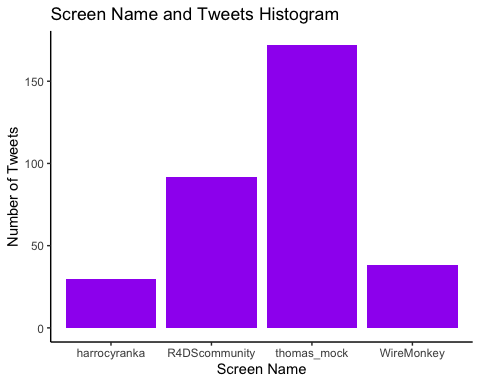
\includegraphics{TidyTuesday_Rtweet_files/figure-latex/unnamed-chunk-5-1.pdf}

\hypertarget{basic-information-on-these-4-accounts.}{%
\paragraph{3. Basic information on these 4
accounts.}\label{basic-information-on-these-4-accounts.}}

Harro Cyranka is working on analytics and data science, political
campaigns, and other cool stuff. His expertise is on predictive
modeling, text mining, data visualization, and app development using R
Shiny. He has some good looking nerdy graphs on his Twitter account.

R4DScommunity is a community of R learners to help learners and mentors
to gather and work through the R for Data Science book by Garrett
Grolemund and Hadley Wickham.

Thomas Mock is fascinated by R, RStudio, the tidyverse, and appreciates
open-source tools in general. He created and runs \#TidyTuesday on
Twitter to help bring the R/Tidyverse concepts to data science
newcomers. He is the co-founder of \#TidyTuesday. His avatar looks good.

Alyssa Goldberg (aka WireMonkey) claims herself as a ``data witch''.
Based on her Tweets, we can tell that she is interested in hierarchical
clustering, internet memes, tidyTuesday, and other things.

\hypertarget{part-ii}{%
\section{Part II}\label{part-ii}}

\hypertarget{install-and-load-the-rtweet-package}{%
\paragraph{2.1 Install and load the rtweet
package}\label{install-and-load-the-rtweet-package}}

\begin{Shaded}
\begin{Highlighting}[]
\KeywordTok{library}\NormalTok{(rtweet)}
\end{Highlighting}
\end{Shaded}

\begin{verbatim}
## 
## Attaching package: 'rtweet'
\end{verbatim}

\begin{verbatim}
## The following object is masked from 'package:purrr':
## 
##     flatten
\end{verbatim}

\hypertarget{use-ts_plot-to-create-a-line-graph-of-the-twitter-data}{%
\paragraph{2.2 Use ts\_plot() to create a line graph of the twitter
data}\label{use-ts_plot-to-create-a-line-graph-of-the-twitter-data}}

\begin{Shaded}
\begin{Highlighting}[]
\KeywordTok{ts_plot}\NormalTok{(df, }\StringTok{"1 weeks"}\NormalTok{) }\OperatorTok{+}\StringTok{ }\KeywordTok{theme_classic}\NormalTok{() }\OperatorTok{+}\StringTok{ }\KeywordTok{theme}\NormalTok{(}\DataTypeTok{plot.title =} \KeywordTok{element_text}\NormalTok{(}\DataTypeTok{face =} \StringTok{"bold"}\NormalTok{)) }\OperatorTok{+}\StringTok{ }\KeywordTok{labs}\NormalTok{(}
    \DataTypeTok{x =} \StringTok{"Months in year"}\NormalTok{, }\DataTypeTok{y =} \StringTok{" Frequency"}\NormalTok{,}
    \DataTypeTok{title =} \StringTok{"Tweets data as a time series"}\NormalTok{,}
    \DataTypeTok{subtitle =} \StringTok{"This graph is created using interval of time expressed as 1 week"}\NormalTok{,}
    \DataTypeTok{caption =} \StringTok{"}\CharTok{\textbackslash{}n}\StringTok{Source: Data collected from #TidyTuesday"}
\NormalTok{  )}
\end{Highlighting}
\end{Shaded}

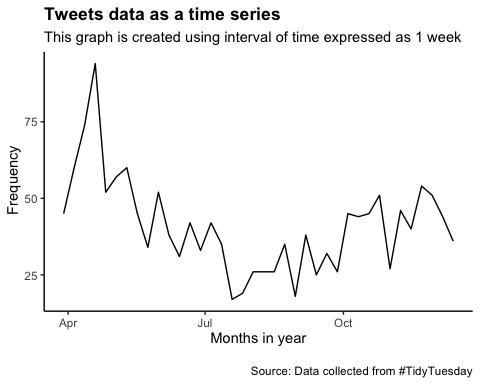
\includegraphics{TidyTuesday_Rtweet_files/figure-latex/unnamed-chunk-7-1.pdf}

\hypertarget{write-a-two-sentence-explanation-of-the-graph.}{%
\paragraph{2.3 Write a two sentence explanation of the
graph.}\label{write-a-two-sentence-explanation-of-the-graph.}}

\emph{Overall, the frequency fluctuates among the timeline. At the
weekly interval, the graph illustrates that the number of tweets reached
highest in between April and May and they dropped right after July and
fluctuated again from August to December. }

\hypertarget{limit-the-data-to-only-the-4-screen-names-in-part-i}{%
\paragraph{2.4 Limit the data to only the 4 screen names in part
I}\label{limit-the-data-to-only-the-4-screen-names-in-part-i}}

\begin{Shaded}
\begin{Highlighting}[]
\NormalTok{df_4names <-}\StringTok{ }\KeywordTok{subset}\NormalTok{(df, screen_name }\OperatorTok{==}\StringTok{ "harrocyranka"}\OperatorTok{|}\NormalTok{screen_name }\OperatorTok{==}\StringTok{ "WireMonkey"}\OperatorTok{|}\NormalTok{screen_name }\OperatorTok{==}\StringTok{ "R4DScommunity"}\OperatorTok{|}\StringTok{ }\NormalTok{screen_name }\OperatorTok{==}\StringTok{ "thomas_mock"}\NormalTok{)}
\CommentTok{#head(df_4names)}
\CommentTok{#tail(df_4names)}
\CommentTok{#str(df_4names)}
\end{Highlighting}
\end{Shaded}

\hypertarget{subset-into-4-individual-screens}{%
\paragraph{2.4.1 Subset into 4 individual
screens}\label{subset-into-4-individual-screens}}

\begin{Shaded}
\begin{Highlighting}[]
\NormalTok{thomas <-}\StringTok{ }\KeywordTok{subset}\NormalTok{(df_4names, screen_name }\OperatorTok{==}\StringTok{"thomas_mock"}\NormalTok{)}
\NormalTok{r4ds <-}\StringTok{ }\KeywordTok{subset}\NormalTok{(df_4names, screen_name }\OperatorTok{==}\StringTok{"R4DScommunity"}\NormalTok{)}
\NormalTok{harro <-}\StringTok{ }\KeywordTok{subset}\NormalTok{(df_4names, screen_name }\OperatorTok{==}\StringTok{"harrocyranka"}\NormalTok{)}
\NormalTok{wiremonkey <-}\StringTok{ }\KeywordTok{subset}\NormalTok{(df_4names, screen_name }\OperatorTok{==}\StringTok{ "WireMonkey"}\NormalTok{)}
\end{Highlighting}
\end{Shaded}

\hypertarget{recreate-the-graph-above-with-the-reduced-data.}{%
\paragraph{2.5 Recreate the graph above with the reduced
data.}\label{recreate-the-graph-above-with-the-reduced-data.}}

\begin{Shaded}
\begin{Highlighting}[]
\KeywordTok{ts_plot}\NormalTok{(df_4names, }\StringTok{"1 weeks"}\NormalTok{) }\OperatorTok{+}\StringTok{ }\KeywordTok{theme_classic}\NormalTok{() }\OperatorTok{+}\StringTok{ }\KeywordTok{theme}\NormalTok{(}\DataTypeTok{plot.title =} \KeywordTok{element_text}\NormalTok{(}\DataTypeTok{face =} \StringTok{"bold"}\NormalTok{)) }\OperatorTok{+}\StringTok{ }\KeywordTok{labs}\NormalTok{(}
    \DataTypeTok{x =} \StringTok{"Months in year"}\NormalTok{, }\DataTypeTok{y =} \StringTok{" Frequency"}\NormalTok{,}
    \DataTypeTok{title =} \StringTok{"Tweets data of Thomas, Harro, WireMonkey, & R4DScommunity as time series"}\NormalTok{,}
    \DataTypeTok{subtitle =} \StringTok{"This graph is created using interval of time expressed as 1 week"}\NormalTok{,}
    \DataTypeTok{caption =} \StringTok{"}\CharTok{\textbackslash{}n}\StringTok{Source: Data collected from #TidyTuesday"}
\NormalTok{  )}
\end{Highlighting}
\end{Shaded}

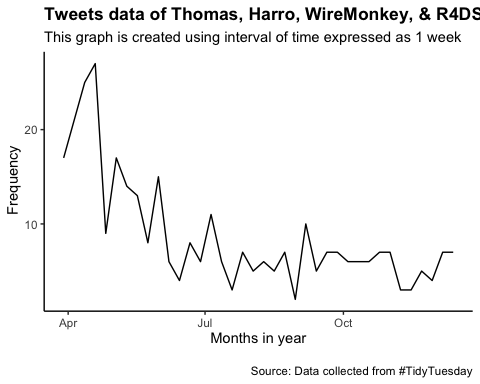
\includegraphics{TidyTuesday_Rtweet_files/figure-latex/unnamed-chunk-10-1.pdf}

\begin{Shaded}
\begin{Highlighting}[]
\KeywordTok{ts_plot}\NormalTok{(thomas,}\StringTok{"1 weeks"}\NormalTok{) }\OperatorTok{+}\StringTok{ }\KeywordTok{theme_classic}\NormalTok{() }\OperatorTok{+}\StringTok{ }\KeywordTok{theme}\NormalTok{(}\DataTypeTok{plot.title =} \KeywordTok{element_text}\NormalTok{(}\DataTypeTok{face =} \StringTok{"bold"}\NormalTok{)) }\OperatorTok{+}\StringTok{ }\KeywordTok{labs}\NormalTok{(}
    \DataTypeTok{x =} \StringTok{"Months in year"}\NormalTok{, }\DataTypeTok{y =} \StringTok{" Frequency"}\NormalTok{,}
    \DataTypeTok{title =} \StringTok{"Tweets data of Thomas"}\NormalTok{,}
    \DataTypeTok{subtitle =} \StringTok{"This graph is created using interval of time expressed as 1 week"}\NormalTok{,}
    \DataTypeTok{caption =} \StringTok{"}\CharTok{\textbackslash{}n}\StringTok{Source: Data collected from #TidyTuesday"}
\NormalTok{  ) }
\end{Highlighting}
\end{Shaded}

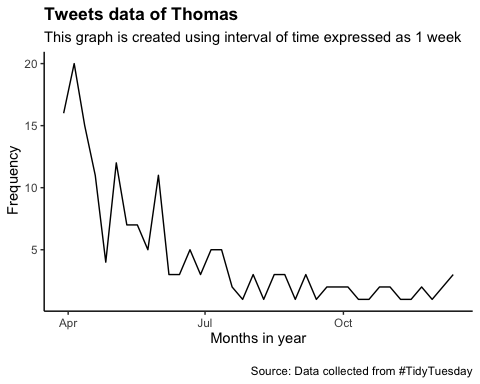
\includegraphics{TidyTuesday_Rtweet_files/figure-latex/unnamed-chunk-11-1.pdf}

\begin{Shaded}
\begin{Highlighting}[]
\KeywordTok{ts_plot}\NormalTok{(r4ds,}\StringTok{"1 weeks"}\NormalTok{) }\OperatorTok{+}\StringTok{ }\KeywordTok{theme_classic}\NormalTok{() }\OperatorTok{+}\StringTok{ }\KeywordTok{theme}\NormalTok{(}\DataTypeTok{plot.title =} \KeywordTok{element_text}\NormalTok{(}\DataTypeTok{face =} \StringTok{"bold"}\NormalTok{)) }\OperatorTok{+}\StringTok{ }\KeywordTok{labs}\NormalTok{(}
    \DataTypeTok{x =} \StringTok{"Months in year"}\NormalTok{, }\DataTypeTok{y =} \StringTok{" Frequency"}\NormalTok{,}
    \DataTypeTok{title =} \StringTok{"Tweets data of R4DS"}\NormalTok{,}
    \DataTypeTok{subtitle =} \StringTok{"This graph is created using interval of time expressed as 1 week"}\NormalTok{,}
    \DataTypeTok{caption =} \StringTok{"}\CharTok{\textbackslash{}n}\StringTok{Source: Data collected from #TidyTuesday"}
\NormalTok{  ) }
\end{Highlighting}
\end{Shaded}

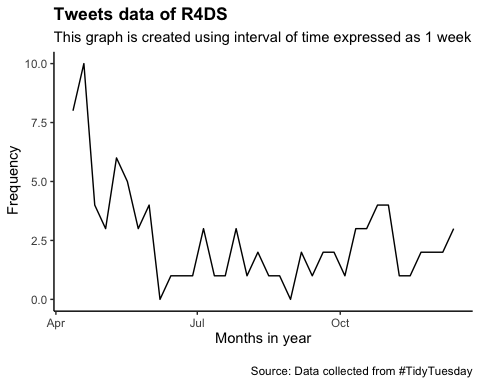
\includegraphics{TidyTuesday_Rtweet_files/figure-latex/unnamed-chunk-12-1.pdf}

\begin{Shaded}
\begin{Highlighting}[]
\KeywordTok{ts_plot}\NormalTok{(harro,}\StringTok{"1 weeks"}\NormalTok{) }\OperatorTok{+}\StringTok{ }\KeywordTok{theme_classic}\NormalTok{() }\OperatorTok{+}\StringTok{ }\KeywordTok{theme}\NormalTok{(}\DataTypeTok{plot.title =} \KeywordTok{element_text}\NormalTok{(}\DataTypeTok{face =} \StringTok{"bold"}\NormalTok{)) }\OperatorTok{+}\StringTok{ }\KeywordTok{labs}\NormalTok{(}
    \DataTypeTok{x =} \StringTok{"Months in year"}\NormalTok{, }\DataTypeTok{y =} \StringTok{" Frequency"}\NormalTok{,}
    \DataTypeTok{title =} \StringTok{"Tweets data of Harro Cyranka"}\NormalTok{,}
    \DataTypeTok{subtitle =} \StringTok{"This graph is created using interval of time expressed as 1 week"}\NormalTok{,}
    \DataTypeTok{caption =} \StringTok{"}\CharTok{\textbackslash{}n}\StringTok{Source: Data collected from #TidyTuesday"}
\NormalTok{  ) }
\end{Highlighting}
\end{Shaded}

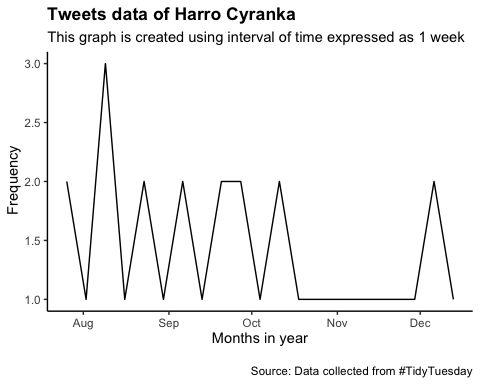
\includegraphics{TidyTuesday_Rtweet_files/figure-latex/unnamed-chunk-13-1.pdf}

\begin{Shaded}
\begin{Highlighting}[]
\KeywordTok{ts_plot}\NormalTok{(wiremonkey,}\StringTok{"1 weeks"}\NormalTok{) }\OperatorTok{+}\StringTok{ }\KeywordTok{theme_classic}\NormalTok{() }\OperatorTok{+}\StringTok{ }\KeywordTok{theme}\NormalTok{(}\DataTypeTok{plot.title =} \KeywordTok{element_text}\NormalTok{(}\DataTypeTok{face =} \StringTok{"bold"}\NormalTok{)) }\OperatorTok{+}\StringTok{ }\KeywordTok{labs}\NormalTok{(}
    \DataTypeTok{x =} \StringTok{"Months in year"}\NormalTok{, }\DataTypeTok{y =} \StringTok{" Frequency"}\NormalTok{,}
    \DataTypeTok{title =} \StringTok{"Tweets data of Wire Monkey"}\NormalTok{,}
    \DataTypeTok{subtitle =} \StringTok{"This graph is created using interval of time expressed as 1 week"}\NormalTok{,}
    \DataTypeTok{caption =} \StringTok{"}\CharTok{\textbackslash{}n}\StringTok{Source: Data collected from #TidyTuesday"}
\NormalTok{  ) }
\end{Highlighting}
\end{Shaded}

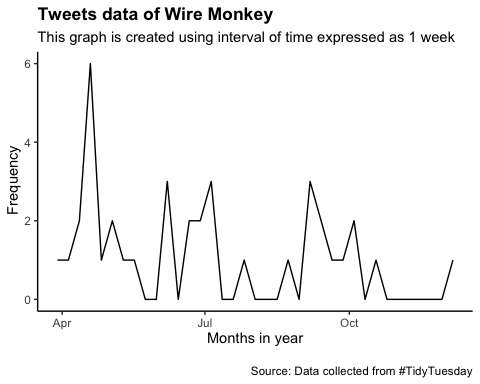
\includegraphics{TidyTuesday_Rtweet_files/figure-latex/unnamed-chunk-14-1.pdf}

\hypertarget{write-a-two-sentence-explanation-of-the-graph.-1}{%
\paragraph{2.6 Write a two sentence explanation of the
graph.}\label{write-a-two-sentence-explanation-of-the-graph.-1}}

\emph{Base on the graphs, it seems that the four examined screennames
were tweeting harmoniously along with the master dataset (df). They are
likely to tweet more around April and May than any other period. }

\hypertarget{use-plain_tweets-to-find-the-top-25-words-tweeted-by-the-4-screen-names.}{%
\paragraph{2.7 Use plain\_tweets() to find the top 25 words tweeted by
the 4 screen
names.}\label{use-plain_tweets-to-find-the-top-25-words-tweeted-by-the-4-screen-names.}}

\begin{Shaded}
\begin{Highlighting}[]
\KeywordTok{library}\NormalTok{(tokenizers) }\CommentTok{#Could not use the tokenize argument, thus I have to install the "Tokenizers" package to do the job.}
\CommentTok{#Convert to plain text}

\NormalTok{thomas_plain <-}\StringTok{ }\KeywordTok{tokenize_words}\NormalTok{(}\KeywordTok{plain_tweets}\NormalTok{(thomas}\OperatorTok{$}\NormalTok{text))}
\NormalTok{r4ds_plain <-}\StringTok{ }\KeywordTok{tokenize_words}\NormalTok{(}\KeywordTok{plain_tweets}\NormalTok{(r4ds}\OperatorTok{$}\NormalTok{text))}
\NormalTok{harro_plain<-}\StringTok{ }\KeywordTok{tokenize_words}\NormalTok{(}\KeywordTok{plain_tweets}\NormalTok{(harro}\OperatorTok{$}\NormalTok{text))}
\NormalTok{wiremonkey_plain <-}\StringTok{ }\KeywordTok{tokenize_words}\NormalTok{(}\KeywordTok{plain_tweets}\NormalTok{(wiremonkey}\OperatorTok{$}\NormalTok{text))}
\end{Highlighting}
\end{Shaded}

\begin{Shaded}
\begin{Highlighting}[]
\NormalTok{count_thomas <-}\StringTok{ }\KeywordTok{table}\NormalTok{(}\KeywordTok{unlist}\NormalTok{(thomas_plain))}
\NormalTok{count_r4ds <-}\StringTok{ }\KeywordTok{table}\NormalTok{(}\KeywordTok{unlist}\NormalTok{(r4ds_plain)) }
\NormalTok{count_harro <-}\StringTok{ }\KeywordTok{table}\NormalTok{(}\KeywordTok{unlist}\NormalTok{(harro_plain)) }
\NormalTok{count_wiremonkey <-}\StringTok{ }\KeywordTok{table}\NormalTok{(}\KeywordTok{unlist}\NormalTok{(wiremonkey_plain)) }
\end{Highlighting}
\end{Shaded}

\emph{Thomas's top 25 words}

\begin{Shaded}
\begin{Highlighting}[]
\NormalTok{thomas_}\DecValTok{25}\NormalTok{ =}\StringTok{ }\KeywordTok{head}\NormalTok{(}\KeywordTok{sort}\NormalTok{(count_thomas, }\DataTypeTok{decreasing =} \OtherTok{TRUE}\NormalTok{), }\DecValTok{25}\NormalTok{)}
\CommentTok{#thomas_25}
\end{Highlighting}
\end{Shaded}

\emph{R4DS's top 25 words}

\begin{Shaded}
\begin{Highlighting}[]
\NormalTok{r4ds_}\DecValTok{25}\NormalTok{ =}\StringTok{ }\KeywordTok{head}\NormalTok{(}\KeywordTok{sort}\NormalTok{(count_r4ds, }\DataTypeTok{decreasing =} \OtherTok{TRUE}\NormalTok{), }\DecValTok{25}\NormalTok{)}
\CommentTok{#r4ds_25}
\end{Highlighting}
\end{Shaded}

\emph{Haro's top 25 words}

\begin{Shaded}
\begin{Highlighting}[]
\NormalTok{harro_}\DecValTok{25}\NormalTok{ =}\StringTok{ }\KeywordTok{head}\NormalTok{(}\KeywordTok{sort}\NormalTok{(count_harro, }\DataTypeTok{decreasing =} \OtherTok{TRUE}\NormalTok{), }\DecValTok{25}\NormalTok{)}
\CommentTok{#harro_25}
\end{Highlighting}
\end{Shaded}

\emph{Wiremonkey's top 25 words}

\begin{Shaded}
\begin{Highlighting}[]
\NormalTok{wiremonkey_}\DecValTok{25}\NormalTok{ =}\StringTok{ }\KeywordTok{head}\NormalTok{(}\KeywordTok{sort}\NormalTok{(count_wiremonkey, }\DataTypeTok{decreasing =} \OtherTok{TRUE}\NormalTok{), }\DecValTok{25}\NormalTok{)}
\CommentTok{#wiremonkey_25}
\end{Highlighting}
\end{Shaded}

\hypertarget{use-the-syuzhet-package-to-conduct-sentiment-analysis.}{%
\paragraph{2.8 Use the syuzhet package to conduct sentiment
analysis.}\label{use-the-syuzhet-package-to-conduct-sentiment-analysis.}}

\hypertarget{tokenizing}{%
\paragraph{2.8.1 Tokenizing}\label{tokenizing}}

\begin{Shaded}
\begin{Highlighting}[]
\KeywordTok{library}\NormalTok{(syuzhet)}
\end{Highlighting}
\end{Shaded}

\begin{verbatim}
## 
## Attaching package: 'syuzhet'
\end{verbatim}

\begin{verbatim}
## The following object is masked from 'package:rtweet':
## 
##     get_tokens
\end{verbatim}

\begin{Shaded}
\begin{Highlighting}[]
\NormalTok{thomas_words <-}\StringTok{ }\KeywordTok{get_tokens}\NormalTok{(thomas}\OperatorTok{$}\NormalTok{text, }\DataTypeTok{pattern =} \StringTok{"}\CharTok{\textbackslash{}\textbackslash{}}\StringTok{W"}\NormalTok{) }
\NormalTok{r4ds_words <-}\StringTok{ }\KeywordTok{get_tokens}\NormalTok{(r4ds}\OperatorTok{$}\NormalTok{text, }\DataTypeTok{pattern =} \StringTok{"}\CharTok{\textbackslash{}\textbackslash{}}\StringTok{W"}\NormalTok{)}
\NormalTok{harro_words <-}\StringTok{ }\KeywordTok{get_tokens}\NormalTok{(harro}\OperatorTok{$}\NormalTok{text, }\DataTypeTok{pattern =} \StringTok{"}\CharTok{\textbackslash{}\textbackslash{}}\StringTok{W"}\NormalTok{)}
\NormalTok{wiremonkey_words <-}\StringTok{ }\KeywordTok{get_tokens}\NormalTok{(wiremonkey}\OperatorTok{$}\NormalTok{text, }\DataTypeTok{pattern =} \StringTok{"}\CharTok{\textbackslash{}\textbackslash{}}\StringTok{W"}\NormalTok{)}
\end{Highlighting}
\end{Shaded}

\hypertarget{conducting-sentiment-analysis-for-each-screen-name-just-use-one-method-named-syuzhet}{%
\paragraph{2.8.2 Conducting sentiment analysis for each screen name
(just use one method named: ``syuzhet''
)}\label{conducting-sentiment-analysis-for-each-screen-name-just-use-one-method-named-syuzhet}}

\begin{Shaded}
\begin{Highlighting}[]
\NormalTok{thomas_syuzhet_vector <-}\StringTok{ }\KeywordTok{get_sentiment}\NormalTok{(thomas_words, }\DataTypeTok{method=}\StringTok{"syuzhet"}\NormalTok{)}
\NormalTok{r4ds_syuzhet_vector <-}\StringTok{ }\KeywordTok{get_sentiment}\NormalTok{(r4ds_words, }\DataTypeTok{method=}\StringTok{"syuzhet"}\NormalTok{)}
\NormalTok{harro_syuzhet_vector <-}\StringTok{ }\KeywordTok{get_sentiment}\NormalTok{(harro_words, }\DataTypeTok{method=}\StringTok{"syuzhet"}\NormalTok{)}
\NormalTok{wiremonkey_syuzhet_vector <-}\StringTok{ }\KeywordTok{get_sentiment}\NormalTok{(wiremonkey_words, }\DataTypeTok{method=}\StringTok{"syuzhet"}\NormalTok{)}

\KeywordTok{sum}\NormalTok{(thomas_syuzhet_vector) }
\end{Highlighting}
\end{Shaded}

\begin{verbatim}
## [1] 239.35
\end{verbatim}

\begin{Shaded}
\begin{Highlighting}[]
\KeywordTok{sum}\NormalTok{(r4ds_syuzhet_vector) }
\end{Highlighting}
\end{Shaded}

\begin{verbatim}
## [1] 83.05
\end{verbatim}

\begin{Shaded}
\begin{Highlighting}[]
\KeywordTok{sum}\NormalTok{(harro_syuzhet_vector) }
\end{Highlighting}
\end{Shaded}

\begin{verbatim}
## [1] 19.8
\end{verbatim}

\begin{Shaded}
\begin{Highlighting}[]
\KeywordTok{sum}\NormalTok{(wiremonkey_syuzhet_vector) }
\end{Highlighting}
\end{Shaded}

\begin{verbatim}
## [1] 13.6
\end{verbatim}

\emph{Thomas's Sentiment Analysis}

\begin{Shaded}
\begin{Highlighting}[]
\KeywordTok{summary}\NormalTok{(thomas_syuzhet_vector)}
\end{Highlighting}
\end{Shaded}

\begin{verbatim}
##     Min.  1st Qu.   Median     Mean  3rd Qu.     Max. 
## -1.00000  0.00000  0.00000  0.04932  0.00000  1.00000
\end{verbatim}

\begin{Shaded}
\begin{Highlighting}[]
\NormalTok{percent_vals_thomas <-}\StringTok{ }\KeywordTok{get_percentage_values}\NormalTok{(thomas_syuzhet_vector, }\DataTypeTok{bins =} \DecValTok{300}\NormalTok{)}

\KeywordTok{plot}\NormalTok{(}
\NormalTok{  percent_vals_thomas, }
  \DataTypeTok{type=}\StringTok{"l"}\NormalTok{, }
  \DataTypeTok{main=}\StringTok{"Thomas's Sentiment Analysis"}\NormalTok{, }
  \DataTypeTok{xlab =} \StringTok{"Narrative Time"}\NormalTok{, }
  \DataTypeTok{ylab=} \StringTok{"Emotional Valence"}
\NormalTok{  )}
\end{Highlighting}
\end{Shaded}

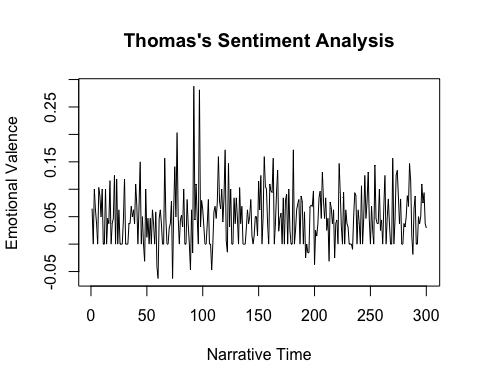
\includegraphics{TidyTuesday_Rtweet_files/figure-latex/unnamed-chunk-24-1.pdf}

\emph{R4DS's Sentiment Analysis}

\begin{Shaded}
\begin{Highlighting}[]
\KeywordTok{summary}\NormalTok{(r4ds_syuzhet_vector)}
\end{Highlighting}
\end{Shaded}

\begin{verbatim}
##    Min. 1st Qu.  Median    Mean 3rd Qu.    Max. 
## -1.0000  0.0000  0.0000  0.0367  0.0000  1.0000
\end{verbatim}

\begin{Shaded}
\begin{Highlighting}[]
\NormalTok{percent_vals_r4ds <-}\StringTok{ }\KeywordTok{get_percentage_values}\NormalTok{(r4ds_syuzhet_vector, }\DataTypeTok{bins =} \DecValTok{300}\NormalTok{)}

\KeywordTok{plot}\NormalTok{(}
\NormalTok{  percent_vals_r4ds, }
  \DataTypeTok{type=}\StringTok{"l"}\NormalTok{, }
  \DataTypeTok{main=}\StringTok{"R4DS's Sentiment Analysis"}\NormalTok{, }
  \DataTypeTok{xlab =} \StringTok{"Narrative Time"}\NormalTok{, }
  \DataTypeTok{ylab=} \StringTok{"Emotional Valence"}
\NormalTok{  )}
\end{Highlighting}
\end{Shaded}

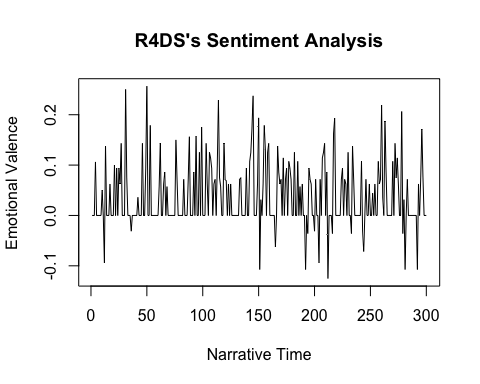
\includegraphics{TidyTuesday_Rtweet_files/figure-latex/unnamed-chunk-26-1.pdf}

\emph{Harro Cyranka's Sentiment Analysis}

\begin{Shaded}
\begin{Highlighting}[]
\KeywordTok{summary}\NormalTok{(harro_syuzhet_vector)}
\end{Highlighting}
\end{Shaded}

\begin{verbatim}
##     Min.  1st Qu.   Median     Mean  3rd Qu.     Max. 
## -1.00000  0.00000  0.00000  0.01568  0.00000  1.00000
\end{verbatim}

\begin{Shaded}
\begin{Highlighting}[]
\NormalTok{percent_vals_harro <-}\StringTok{ }\KeywordTok{get_percentage_values}\NormalTok{(harro_syuzhet_vector, }\DataTypeTok{bins =} \DecValTok{300}\NormalTok{)}

\KeywordTok{plot}\NormalTok{(}
\NormalTok{  percent_vals_harro, }
  \DataTypeTok{type=}\StringTok{"l"}\NormalTok{, }
  \DataTypeTok{main=}\StringTok{"Harro Cyranka's Sentiment Analysis"}\NormalTok{, }
  \DataTypeTok{xlab =} \StringTok{"Narrative Time"}\NormalTok{, }
  \DataTypeTok{ylab=} \StringTok{"Emotional Valence"}
\NormalTok{  )}
\end{Highlighting}
\end{Shaded}

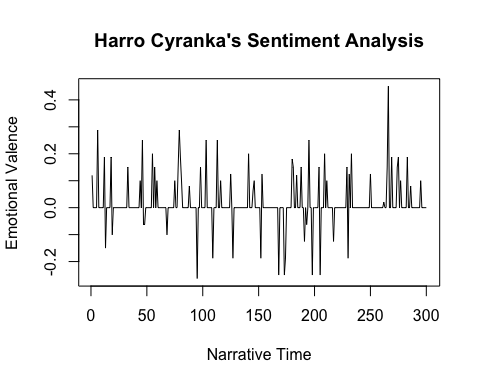
\includegraphics{TidyTuesday_Rtweet_files/figure-latex/unnamed-chunk-28-1.pdf}

\emph{Wire Monkey's Sentiment Analysis}

\begin{Shaded}
\begin{Highlighting}[]
\KeywordTok{summary}\NormalTok{(wiremonkey_syuzhet_vector)}
\end{Highlighting}
\end{Shaded}

\begin{verbatim}
##      Min.   1st Qu.    Median      Mean   3rd Qu.      Max. 
## -0.800000  0.000000  0.000000  0.008889  0.000000  1.000000
\end{verbatim}

\begin{Shaded}
\begin{Highlighting}[]
\NormalTok{percent_vals_wiremonkey <-}\StringTok{ }\KeywordTok{get_percentage_values}\NormalTok{(wiremonkey_syuzhet_vector, }\DataTypeTok{bins =} \DecValTok{300}\NormalTok{)}

\KeywordTok{plot}\NormalTok{(}
\NormalTok{  percent_vals_wiremonkey, }
  \DataTypeTok{type=}\StringTok{"l"}\NormalTok{, }
  \DataTypeTok{main=}\StringTok{"Wire Monkey's Sentiment Analysis"}\NormalTok{, }
  \DataTypeTok{xlab =} \StringTok{"Narrative Time"}\NormalTok{, }
  \DataTypeTok{ylab=} \StringTok{"Emotional Valence"}
\NormalTok{  )}
\end{Highlighting}
\end{Shaded}

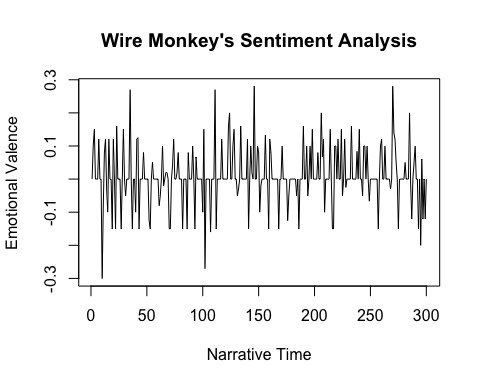
\includegraphics{TidyTuesday_Rtweet_files/figure-latex/unnamed-chunk-30-1.pdf}

\hypertarget{comment-about-the-graphs-write-a-two-sentence-explanation-of-the-graph}{%
\paragraph{Comment about the graphs (Write a two sentence explanation of
the
graph):}\label{comment-about-the-graphs-write-a-two-sentence-explanation-of-the-graph}}

\emph{No screen names have negative sentiment scores and the general
average scores are slightly higher than 0. Among the four screen names,
Thomas has the highest average sentiment score (0.04932) while the
lowest average score belongs to Wire Monkey (0.04932). R4DS and Harro
have average scores of 0.0367 and 0.01568, respectively. }

\hypertarget{separate-the-data-into-2-dataframes-include-hadleywickham-and-do-not}{%
\paragraph{2.9 Separate the data into 2 dataframes: include
@hadleywickham and do
not}\label{separate-the-data-into-2-dataframes-include-hadleywickham-and-do-not}}

\begin{Shaded}
\begin{Highlighting}[]
\NormalTok{wickham =}\StringTok{ }\KeywordTok{subset}\NormalTok{(df, }\KeywordTok{grepl}\NormalTok{(}\StringTok{"hadleywickham"}\NormalTok{, mentions_screen_name))}
\CommentTok{#wickham}
\CommentTok{#21 of them do mention wickham  }
\end{Highlighting}
\end{Shaded}

\begin{Shaded}
\begin{Highlighting}[]
\NormalTok{no_wickham =}\StringTok{ }\KeywordTok{subset}\NormalTok{(df, }\OperatorTok{!}\KeywordTok{grepl}\NormalTok{(}\StringTok{"hadleywickham"}\NormalTok{, mentions_screen_name))}
\CommentTok{#head(no_wickham)}
\CommentTok{#tail(no_wickham)}
\CommentTok{#str(no_wickham)}

\CommentTok{#no_wickham # 1544 tweets that don't mention Wickham }
\end{Highlighting}
\end{Shaded}

\hypertarget{conduct-sentiment-analysis-on-the-two-datasets.}{%
\paragraph{2.10 Conduct sentiment analysis on the two
datasets.}\label{conduct-sentiment-analysis-on-the-two-datasets.}}

\hypertarget{tweets-that-mentions-wickham-sentiment-analysis}{%
\subparagraph{2.10.1 Tweets that mentions Wickham Sentiment
Analysis}\label{tweets-that-mentions-wickham-sentiment-analysis}}

\begin{Shaded}
\begin{Highlighting}[]
\NormalTok{wickham_words <-}\StringTok{ }\KeywordTok{get_tokens}\NormalTok{(wickham}\OperatorTok{$}\NormalTok{text, }\DataTypeTok{pattern =} \StringTok{"}\CharTok{\textbackslash{}\textbackslash{}}\StringTok{W"}\NormalTok{) }\CommentTok{#tokenize into single words}
\CommentTok{#str(wickham_words)}
\NormalTok{wickham_syuzhet_vector <-}\StringTok{ }\KeywordTok{get_sentiment}\NormalTok{(wickham_words, }\DataTypeTok{method=}\StringTok{"syuzhet"}\NormalTok{)}
\KeywordTok{str}\NormalTok{(wickham_syuzhet_vector)}
\end{Highlighting}
\end{Shaded}

\begin{verbatim}
##  num [1:750] 0 0 0 0 0 0 0 0 0 0 ...
\end{verbatim}

\begin{Shaded}
\begin{Highlighting}[]
\KeywordTok{summary}\NormalTok{(wickham_syuzhet_vector)}
\end{Highlighting}
\end{Shaded}

\begin{verbatim}
##    Min. 1st Qu.  Median    Mean 3rd Qu.    Max. 
## -1.0000  0.0000  0.0000  0.0374  0.0000  1.0000
\end{verbatim}

2.10.2 Tweets that Mentions do not mention Wickham Sentiment Analysis

\begin{Shaded}
\begin{Highlighting}[]
\NormalTok{no_wickham_words <-}\StringTok{ }\KeywordTok{get_tokens}\NormalTok{(no_wickham}\OperatorTok{$}\NormalTok{text, }\DataTypeTok{pattern =} \StringTok{"}\CharTok{\textbackslash{}\textbackslash{}}\StringTok{W"}\NormalTok{) }\CommentTok{#tokenize into single words}
\CommentTok{#no_wickham_words}
\NormalTok{no_wickham_syuzhet_vector <-}\StringTok{ }\KeywordTok{get_sentiment}\NormalTok{(no_wickham_words, }\DataTypeTok{method=}\StringTok{"syuzhet"}\NormalTok{)}
\KeywordTok{str}\NormalTok{(no_wickham_syuzhet_vector)}
\end{Highlighting}
\end{Shaded}

\begin{verbatim}
##  num [1:48591] 0 0 0 0 0 0 0 0 0 0 ...
\end{verbatim}

\begin{Shaded}
\begin{Highlighting}[]
\KeywordTok{summary}\NormalTok{(no_wickham_syuzhet_vector)}
\end{Highlighting}
\end{Shaded}

\begin{verbatim}
##     Min.  1st Qu.   Median     Mean  3rd Qu.     Max. 
## -1.00000  0.00000  0.00000  0.02541  0.00000  1.00000
\end{verbatim}

2.10.3 Combine two vectors together and convert it to a dataframe

\begin{Shaded}
\begin{Highlighting}[]
\NormalTok{combined =}\StringTok{ }\KeywordTok{cbind}\NormalTok{(no_wickham_syuzhet_vector,wickham_syuzhet_vector)}
\end{Highlighting}
\end{Shaded}

\begin{verbatim}
## Warning in cbind(no_wickham_syuzhet_vector, wickham_syuzhet_vector): number
## of rows of result is not a multiple of vector length (arg 2)
\end{verbatim}

\begin{Shaded}
\begin{Highlighting}[]
\NormalTok{combined =}\StringTok{ }\KeywordTok{as.data.frame}\NormalTok{(combined)}
\CommentTok{#head(combined)}
\CommentTok{#tail(combined)}
\CommentTok{#str(combined)}
\end{Highlighting}
\end{Shaded}

\hypertarget{make-the-data-frame-easy-to-conduct-the-t-test}{%
\subparagraph{2.10.4 Make the data frame easy to conduct the
t-test}\label{make-the-data-frame-easy-to-conduct-the-t-test}}

\begin{Shaded}
\begin{Highlighting}[]
\NormalTok{df_combined <-}\StringTok{ }\KeywordTok{gather}\NormalTok{(combined, }\DataTypeTok{key=}\StringTok{"measure"}\NormalTok{, }\DataTypeTok{value=}\StringTok{"value"}\NormalTok{, }\KeywordTok{c}\NormalTok{(}\StringTok{"no_wickham_syuzhet_vector"}\NormalTok{, }\StringTok{"wickham_syuzhet_vector"}\NormalTok{))}
\CommentTok{#head(df_combined)}
\CommentTok{#tail(df_combined)}
\CommentTok{#str(df_combined)}
\end{Highlighting}
\end{Shaded}

\emph{Calculate mean and standard deviation}

\begin{Shaded}
\begin{Highlighting}[]
\NormalTok{df_combined}\OperatorTok\StringTok{ }\KeywordTok{group_by}\NormalTok{(measure) }\OperatorTok\StringTok{  }\KeywordTok{summarize}\NormalTok{(}\DataTypeTok{Program_sd =} \KeywordTok{sd}\NormalTok{(value))}
\end{Highlighting}
\end{Shaded}

\begin{verbatim}
## # A tibble: 2 x 2
##   measure                   Program_sd
##   <chr>                          <dbl>
## 1 no_wickham_syuzhet_vector      0.176
## 2 wickham_syuzhet_vector         0.190
\end{verbatim}

\begin{Shaded}
\begin{Highlighting}[]
\NormalTok{df_combined}\OperatorTok\StringTok{ }\KeywordTok{group_by}\NormalTok{(measure) }\OperatorTok\StringTok{  }\KeywordTok{summarize}\NormalTok{(}\DataTypeTok{Mean =} \KeywordTok{mean}\NormalTok{(value))}
\end{Highlighting}
\end{Shaded}

\begin{verbatim}
## # A tibble: 2 x 2
##   measure                     Mean
##   <chr>                      <dbl>
## 1 no_wickham_syuzhet_vector 0.0254
## 2 wickham_syuzhet_vector    0.0374
\end{verbatim}

\hypertarget{run-a-t-test-on-to-see-include-hadleywickham-are-more-or-less-positive-than-tweets-without.}{%
\paragraph{2.11 Run a t-test on to see include @hadleywickham are more
or less positive than tweets
without.}\label{run-a-t-test-on-to-see-include-hadleywickham-are-more-or-less-positive-than-tweets-without.}}

\begin{Shaded}
\begin{Highlighting}[]
\NormalTok{ind.t.test<-}\KeywordTok{t.test}\NormalTok{(value }\OperatorTok{~}\StringTok{ }\NormalTok{measure, }\DataTypeTok{data =}\NormalTok{ df_combined)}
\NormalTok{ind.t.test}
\end{Highlighting}
\end{Shaded}

\begin{verbatim}
## 
##  Welch Two Sample t-test
## 
## data:  value by measure
## t = -10.188, df = 96602, p-value < 2.2e-16
## alternative hypothesis: true difference in means is not equal to 0
## 95 percent confidence interval:
##  -0.014280459 -0.009672536
## sample estimates:
## mean in group no_wickham_syuzhet_vector 
##                              0.02541314 
##    mean in group wickham_syuzhet_vector 
##                              0.03738964
\end{verbatim}

\begin{Shaded}
\begin{Highlighting}[]
\CommentTok{#str(ind.t.test)}
\end{Highlighting}
\end{Shaded}

\hypertarget{report-t-test}{%
\paragraph{Report t-test}\label{report-t-test}}

\begin{Shaded}
\begin{Highlighting}[]
\CommentTok{#str(summary(ind.t.test))}
\NormalTok{pval <-}\StringTok{ }\NormalTok{ind.t.test}\OperatorTok{$}\NormalTok{p.value}
\NormalTok{tval <-}\StringTok{ }\NormalTok{ind.t.test}\OperatorTok{$}\NormalTok{statistic}
\end{Highlighting}
\end{Shaded}

The 21 tweets that mention Hadley Wickham (M = 0.0374, SD = 0.1901793 )
compared to the 1544 tweets that do not mention Hadley Wickham (M =
0.02541, SD = 0.1759960) demonstrated significantly better sentiment
scores, t(96602) = -10.18845 , p = \ensuremath{2.297258\times 10^{-24}}


\end{document}
